\documentclass[11pt,a4paper]{report}

% --- Required Packages ---
\usepackage[utf8]{inputenc}
\usepackage{amsmath}
\usepackage{amssymb}
\usepackage{tikz}
\usepackage{algorithm}
\usepackage{algpseudocode}
\usepackage{hyperref} % For clickable links in the table of contents

% --- Document Start ---
\begin{document}

\tableofcontents
\vspace{2em}

%%%%%%%%%%%%%%%%%%%%%%%%%%%%%%%%%%%%%%%%%%%%%%%%%%%%%%%%%%%%%%%%%%%%%%%%%%%%%%
\chapter{Conceptual summary: what sparse grids do and why they matter}

Classical tensor-product discretizations for a PDE on $\Omega=(0,1)^d$ suffer from the curse of dimensionality: if one uses $N$ degrees of freedom per coordinate direction, then the total number of unknowns scales like $N^d$. Sparse grids exploit a specific kind of smoothness --- bounded mixed derivatives --- to replace this full tensor-product construction by a carefully truncated multilevel tensor product. The result is a discretization whose number of degrees of freedom is reduced to
$$
O\!\bigl(N(\log N)^{d-1}\bigr),
$$
while the approximation error for piecewise multilinear approximation deteriorates only by a logarithmic factor compared with the full grid.

The key idea is hierarchical decomposition. In one dimension, piecewise linear finite element spaces can be decomposed into increment spaces $W_l$, where level $l$ resolves structures on mesh width $h_l=2^{-l}$. In several dimensions, one takes tensor products $W_{l_1}\otimes\cdots\otimes W_{l_d}$, indexed by a multi-index $l=(l_1,\dots,l_d)$. A full grid keeps all subspaces with $|l|_\infty\le n$. A sparse grid keeps only those with
$$
|l|_1 \le n+d-1.
$$
Geometrically, this replaces the full ``box'' of active subspaces in level space by a simplex. Intuitively, highly anisotropic subspaces with one or two fine directions and several coarse directions are cheap and useful, while simultaneously very fine resolution in all directions is too expensive relative to the additional benefit.

Why does this work? For functions $u$ with bounded mixed second derivatives, the hierarchical coefficients decay rapidly with level:
$$
|v_{l,i}| = O(2^{-2|l|_1}),
$$
whereas the number of basis functions on level $l$ grows like
$$
|W_l| = O(2^{|l|_1}).
$$
Thus the ``benefit per cost'' decreases strongly as $|l|_1$ grows, which motivates truncating the tensor expansion by total level rather than by maximal level. This is the core Smolyak/sparse-grid principle.

For PDEs, one can use sparse grids in at least two closely related ways. The first is a direct sparse-grid discretization, for example by a Galerkin finite element method in the sparse space $\widehat V_n$. The second is the combination technique: solve the PDE on several anisotropic full grids and combine those solutions linearly so as to reproduce the sparse-grid approximation to leading order. The direct method gives a conceptually clean variational formulation; the combination technique is often easier to implement on top of existing full-grid solvers and parallelizes very well.

For diffusion-type parabolic problems --- heat equations, Fokker--Planck equations in suitably smooth settings, and related linear evolution equations --- sparse grids are attractive because the spatial operator is elliptic and the solution is often smooth enough in mixed directions away from singularities. In the natural energy norm, sparse grids are particularly effective: there are energy-based sparse-grid variants whose complexity is essentially $O(N)$ for $O(N^{-1})$-type accuracy. This makes sparse grids one of the main deterministic approaches for moderate to fairly high-dimensional PDEs when the solution structure is anisotropic but still smooth enough to justify mixed-derivative approximation estimates.

%%%%%%%%%%%%%%%%%%%%%%%%%%%%%%%%%%%%%%%%%%%%%%%%%%%%%%%%%%%%%%%%%%%%%%%%%%%%%%
\chapter{How sparse grids work: a technical exposition}

\section{The problem setting}

We consider approximation and PDE discretization on the $d$-dimensional unit cube
$$
\Omega := (0,1)^d,
$$
with homogeneous Dirichlet boundary conditions for simplicity. The sparse-grid construction is most naturally motivated for functions whose \emph{mixed} derivatives are controlled. A standard model class is
$$
X^{0}_{q,2}(\Omega)
:=
\left\{
u:\Omega\to\mathbb{R}\;:\;
D^\alpha u \in L^q(\Omega)\ \text{for all } |\alpha|_\infty\le 2,\;
u|_{\partial\Omega}=0
\right\},
$$
with $q=2$ or $q=\infty$. Equivalently, one often formulates the theory in the mixed Sobolev space $H^2_{\mathrm{mix}}(\Omega)$.

The point is not that sparse grids magically defeat dimensionality for arbitrary high-dimensional functions. Rather, they exploit an anisotropic regularity assumption: many high-dimensional functions arising from diffusion-like equations are not extremely smooth in the isotropic sense, but they may still have bounded \emph{mixed} derivatives up to moderate order. Sparse-grid approximation is tailored exactly to that situation.

\section{One-dimensional multilevel decomposition}

\subsection{Grid hierarchy and nodal basis}

For each level $l\in\mathbb{N}$, define the mesh width
$$
h_l := 2^{-l},
$$
and the one-dimensional grid
$$
\Omega_l := \{x_{l,i}=i h_l : 0\le i\le 2^l\}.
$$
As basic building block we use the standard hat function
$$
\varphi(x)=
\begin{cases}
1-|x|, & |x|\le 1,\\
0, & |x|>1.
\end{cases}
$$
Its scaled/shifted copies are
$$
\varphi_{l,i}(x)
=
\varphi\!\left(\frac{x-i h_l}{h_l}\right),
\qquad 1\le i\le 2^l-1.
$$
The corresponding finite element space is
$$
V_l := \mathrm{span}\{\varphi_{l,i} : 1\le i\le 2^l-1\},
$$
the usual space of piecewise linear functions vanishing at the boundary.

\subsection{Hierarchical increment spaces}

Instead of working directly with the nested spaces
$$
V_1 \subset V_2 \subset \cdots,
$$
we decompose them into hierarchical increments. Define
$$
I_l := \{\, i\in\mathbb{N} : 1\le i\le 2^l-1,\ i\ \text{odd}\,\},
$$
and
$$
W_l := \mathrm{span}\{\varphi_{l,i}: i\in I_l\}.
$$
Then one has the direct-sum type decomposition
$$
V_l = \bigoplus_{k=1}^l W_k.
$$
Every $u\in V_l$ therefore admits a hierarchical representation
$$
u(x)=\sum_{k=1}^l \sum_{i\in I_k} v_{k,i}\,\varphi_{k,i}(x),
$$
where $v_{k,i}$ are the \emph{hierarchical surpluses}. These coefficients measure how much genuinely new information is added at level $k$.

A very useful way to interpret the surplus is:
$$
v_{l,i}
=
u(x_{l,i}) - \text{(interpolation from coarser levels at }x_{l,i}\text{)}.
$$
Hence the surplus is small if the coarser representation already predicts the function well at that point.

\subsection{Why hierarchy matters}

In a nodal basis, all grid values are treated symmetrically. In a hierarchical basis, the coefficient size carries information about local scale and, in adaptive variants, about local importance. This is one of the structural reasons sparse grids are possible at all: one can rank subspaces by scale and contribution.

\begin{figure}[ht]
\centering
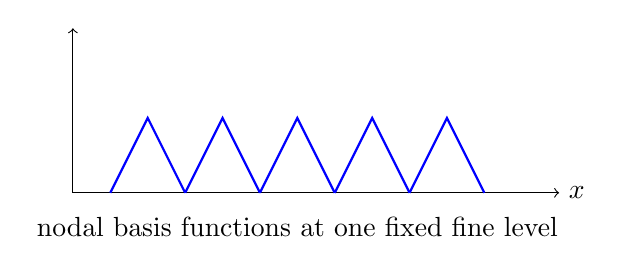
\begin{tikzpicture}[scale=0.95]
\draw[->] (0,0) -- (6.5,0) node[right] {$x$};
\draw[->] (0,0) -- (0,2.2);

% nodal-ish level 3
\begin{scope}[shift={(0,0)}]
\draw[thick,blue] (0.5,0) -- (1.0,1) -- (1.5,0);
\draw[thick,blue] (1.5,0) -- (2.0,1) -- (2.5,0);
\draw[thick,blue] (2.5,0) -- (3.0,1) -- (3.5,0);
\draw[thick,blue] (3.5,0) -- (4.0,1) -- (4.5,0);
\draw[thick,blue] (4.5,0) -- (5.0,1) -- (5.5,0);
\node at (3,-0.45) {nodal basis functions at one fixed fine level};
\end{scope}
\end{tikzpicture}
\caption{Schematic one-dimensional hat functions on a fine level. In the hierarchical construction one splits the nested nodal spaces into increment spaces $W_l$, keeping only the odd-index basis functions as new degrees of freedom on level $l$.}
\label{fig:1d-hats}
\end{figure}

\section{Tensor-product construction in several dimensions}

\subsection{Multivariate grids and basis functions}

Let $l=(l_1,\dots,l_d)\in\mathbb{N}^d$ be a multi-index. Define
$$
h_l := (2^{-l_1},\dots,2^{-l_d}),
\qquad
x_{l,i} := (i_1 2^{-l_1},\dots,i_d 2^{-l_d}).
$$
The tensor-product basis functions are
$$
\varphi_{l,i}(x)
=
\prod_{j=1}^d \varphi_{l_j,i_j}(x_j),
\qquad x=(x_1,\dots,x_d).
$$
The corresponding tensor-product finite element space is
$$
V_l := \mathrm{span}\{\varphi_{l,i}: 1\le i \le 2^l-1\},
$$
and the multivariate hierarchical increment space is
$$
W_l := \mathrm{span}\{\varphi_{l,i}: i\in I_l\},
$$
where
$$
I_l
=
\left\{
i\in\mathbb{N}^d:\ 1\le i \le 2^l-1,\ \text{and each } i_j \text{ is odd}
\right\}.
$$
Again,
$$
V_l = \bigoplus_{k\le l} W_k,
$$
with componentwise ordering.

Hence any sufficiently regular function admits a multilevel expansion
$$
u(x)
=
\sum_{l\in\mathbb{N}^d} \sum_{i\in I_l} v_{l,i}\,\varphi_{l,i}(x)
=
\sum_{l\in\mathbb{N}^d} u_l(x),
\qquad
u_l\in W_l.
$$

\subsection{Cost of one subspace}

The number of basis functions in $W_l$ is
$$
\dim W_l = |I_l| = \prod_{j=1}^d 2^{l_j-1} = 2^{|l|_1-d},
$$
so, up to constants,
$$
\dim W_l \asymp 2^{|l|_1}.
$$
Thus the cost of a subspace grows exponentially in the total level $|l|_1$.

\subsection{Decay of hierarchical coefficients}

For functions with bounded mixed second derivatives, the hierarchical surpluses satisfy
$$
|v_{l,i}| = O(2^{-2|l|_1}).
$$
This is the decisive estimate. It says that the information carried by level $l$ decays much faster than the number of coefficients on that level grows. Roughly:
$$
\text{cost}(W_l)\asymp 2^{|l|_1},
\qquad
\text{benefit}(W_l)\asymp 2^{-2|l|_1}.
$$
So the total contribution of deep levels decreases strongly with $|l|_1$, which suggests selecting subspaces by a \emph{total-level} cut-off.

\section{From full grids to sparse grids}

\subsection{Full-grid space}

If one fixes a maximal one-dimensional level $n$ in each coordinate, one obtains the classical full tensor-product space
$$
V_n^{\mathrm{full}}
=
\bigoplus_{|l|_\infty\le n} W_l.
$$
Its dimension behaves like
$$
\dim V_n^{\mathrm{full}} \asymp 2^{nd}.
$$
This is the usual curse of dimensionality.

\subsection{Classical sparse-grid space}

The classical sparse-grid space keeps only the subspaces satisfying
$$
|l|_1 \le n+d-1.
$$
Thus one defines
$$
\widehat V_n
:=
\bigoplus_{|l|_1\le n+d-1} W_l.
$$
This is the canonical Smolyak-type sparse space for piecewise multilinear approximation.

Its dimension satisfies
$$
\dim \widehat V_n
=
\sum_{i=0}^{n-1} 2^i \binom{d-1+i}{d-1}
=
O(2^n n^{d-1}).
$$
Since $h_n=2^{-n}$, this is equivalently
$$
\dim \widehat V_n = O\!\bigl(h_n^{-1} |\log h_n|^{d-1}\bigr).
$$

For $u\in H^2_{\mathrm{mix}}(\Omega)$, the interpolation error of the sparse-grid interpolant $\widehat u_n\in\widehat V_n$ satisfies
$$
\|u-\widehat u_n\|_{L^2(\Omega)}
=
O(h_n^2 n^{d-1}),
\qquad
\|u-\widehat u_n\|_{L^\infty(\Omega)}
=
O(h_n^2 n^{d-1}).
$$
Thus, compared with the full-grid error $O(h_n^2)$, one loses only a logarithmic factor.

\subsection{Geometric picture in level space}

A very useful way to understand sparse grids is to draw the active subspaces $W_l$ in the integer lattice of level indices. In $d=2$, the full grid keeps a square of indices; the sparse grid keeps a lower simplex.

\begin{figure}[ht]
\centering
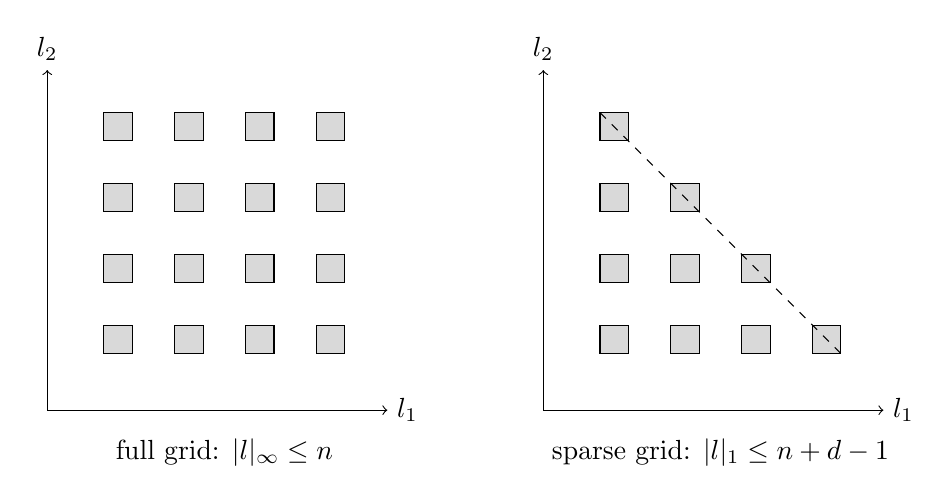
\begin{tikzpicture}[scale=0.9]
% left: full grid
\begin{scope}
\draw[->] (0,0) -- (4.8,0) node[right] {$l_1$};
\draw[->] (0,0) -- (0,4.8) node[above] {$l_2$};
\foreach \x in {1,2,3,4}
  \foreach \y in {1,2,3,4}
    \draw[fill=gray!30] (\x-0.2,\y-0.2) rectangle (\x+0.2,\y+0.2);
\node at (2.5,-0.6) {full grid: $|l|_\infty\le n$};
\end{scope}

% right: sparse grid
\begin{scope}[shift={(7,0)}]
\draw[->] (0,0) -- (4.8,0) node[right] {$l_1$};
\draw[->] (0,0) -- (0,4.8) node[above] {$l_2$};
\foreach \x in {1,2,3,4}
  \foreach \y in {1,2,3,4}
    {
      \pgfmathparse{(\x+\y<=5)?1:0}
      \ifnum\pgfmathresult=1
        \draw[fill=gray!30] (\x-0.2,\y-0.2) rectangle (\x+0.2,\y+0.2);
      \fi
    }
\draw[dashed] (0.8,4.2)--(4.2,0.8);
\node at (2.5,-0.6) {sparse grid: $|l|_1\le n+d-1$};
\end{scope}
\end{tikzpicture}
\caption{Active subspaces in level space. The sparse grid discards the high-cost/high-level corner where all directions are simultaneously fine.}
\label{fig:level-set}
\end{figure}

\section{Why the sparse-grid cut-off is natural}

The sparse-grid selection can be derived by an a priori cost--benefit analysis.

Let
$$
c_l \asymp \dim W_l \asymp 2^{|l|_1},
$$
and let $b_l$ denote an upper bound for the contribution of $u_l$ to the approximation error. From mixed-derivative estimates one gets
$$
b_l \asymp 2^{-2|l|_1}
$$
in $L^\infty$ or $L^2$, up to constants. Hence the local cost--benefit ratio behaves like
$$
\frac{b_l}{c_l} \asymp 2^{-3|l|_1}.
$$
Therefore one should include first all subspaces with small $|l|_1$, then progressively larger total levels. This exactly yields the simplex-type truncation
$$
|l|_1 \le n+d-1.
$$

This derivation matters conceptually: sparse grids are not merely a geometric trick, but an optimization of which anisotropic subspaces are most valuable under a mixed-regularity assumption.

\section{Interpolation error estimates}

The sparse-grid interpolant $\widehat u_n\in \widehat V_n$ is obtained by truncating the hierarchical expansion:
$$
\widehat u_n
=
\sum_{|l|_1\le n+d-1} u_l.
$$
Hence
$$
u-\widehat u_n
=
\sum_{|l|_1>n+d-1} u_l.
$$
The error is therefore controlled by summing the neglected subspace contributions. Using bounds of the form
$$
\|u_l\|_{L^2} \lesssim 2^{-2|l|_1},
\qquad
\|u_l\|_{L^\infty} \lesssim 2^{-2|l|_1},
$$
and counting how many indices satisfy $|l|_1=m$, one obtains the classical bounds
$$
\|u-\widehat u_n\|_{L^2}
=
O(2^{-2n} n^{d-1}),
\qquad
\|u-\widehat u_n\|_{L^\infty}
=
O(2^{-2n} n^{d-1}).
$$
The polynomial factor $n^{d-1}$ is the price paid for the boundary size of the simplex in level space.

\section{The energy norm}

\subsection{Definition and relevance}

For elliptic and parabolic PDEs, the most natural norm is often the energy norm
$$
\|v\|_E
:=
\left(
\sum_{j=1}^d \|\partial_{x_j} v\|_{L^2(\Omega)}^2
\right)^{1/2}.
$$
In $H_0^1(\Omega)$, this is equivalent to the $H^1$-norm. For diffusion operators, the bilinear form of the PDE controls exactly this quantity (or an equivalent weighted version of it), so error estimates in energy norm are especially meaningful.

\subsection{Subspace estimates in energy norm}

For hierarchical subspace components $u_l\in W_l$, one obtains bounds of the type
$$
\|u_l\|_E
\lesssim
2^{-2|l|_1}
\left(
\sum_{j=1}^d 2^{2l_j}
\right)^{1/2}.
$$
Compared with the $L^2$ estimate, the factor $\left(\sum_j 2^{2l_j}\right)^{1/2}$ reflects the presence of first derivatives. Fine resolution in one direction is therefore penalized more strongly in the energy norm than in $L^2$.

\subsection{Classical sparse grid in energy norm}

Even the classical sparse grid already gives
$$
\|u-\widehat u_n\|_E = O(h_n),
$$
that is, the same order in $h_n$ as the full-grid piecewise linear method. This is an important and sometimes underappreciated point: while the $L^2$ and $L^\infty$ errors incur logarithmic losses, the energy norm retains first-order accuracy.

\subsection{Energy-based sparse grids}

One can go further and optimize the index set specifically for the energy norm. The resulting space is smaller than the classical sparse-grid space and roughly selects subspaces according to the criterion
$$
|l|_1 - \frac{1}{5}\log_2\!\left(\prod_{j=1}^d 4^{l_j}\right)
\le n+d-1 - \frac{1}{5}\log_2(4^n 4^{d-1}),
$$
which is the energy-based analogue of the simple total-level cut-off.

The key consequence is:
$$
\dim V_n^{(E)} = O(2^n)=O(h_n^{-1}),
\qquad
\|u-u_n^{(E)}\|_E = O(2^{-n})=O(h_n).
$$
Thus the $n$-dependent complexity in the energy norm no longer carries the factor $n^{d-1}$. In that precise sense, the curse of dimensionality disappears from the \emph{order} of the complexity, even though the hidden constants still depend on $d$.

\subsection{Interpretation}

For diffusion-type PDEs, this is one of the strongest arguments in favor of sparse grids. The variational formulation already lives in $H_0^1$, and sparse grids are especially economical in exactly that norm.

\section{Galerkin discretization on sparse grids}

\subsection{Variational formulation}

Consider a symmetric elliptic operator
$$
\mathcal{L}u = -\nabla\cdot (A(x)\nabla u) + c(x)u
$$
with $A(x)$ uniformly positive definite and $c(x)\ge 0$. The weak formulation reads:

Find $u\in H_0^1(\Omega)$ such that
$$
a(u,v) = (f,v)
\qquad\text{for all } v\in H_0^1(\Omega),
$$
where
$$
a(u,v) = \int_\Omega \nabla v^\top A(x)\nabla u\,dx + \int_\Omega c(x)uv\,dx.
$$

The sparse-grid Galerkin approximation is:

Find $u_n\in \widehat V_n$ such that
$$
a(u_n,v_n) = (f,v_n)
\qquad\text{for all } v_n\in \widehat V_n.
$$

If $\{\phi_\lambda\}_{\lambda\in\Lambda_n}$ is a basis of $\widehat V_n$, then with
$$
u_n = \sum_{\lambda\in\Lambda_n} U_\lambda \phi_\lambda,
$$
one obtains the linear system
$$
K U = F,
$$
where
$$
K_{\lambda\mu} = a(\phi_\mu,\phi_\lambda),
\qquad
F_\lambda = (f,\phi_\lambda).
$$

\subsection{Why this is nontrivial}

Sparse-grid finite element spaces are not tensor-product spaces in the ordinary sense; they are sums of anisotropic tensor-product subspaces. This complicates basis handling, assembly, and linear solvers. However, the hierarchical construction also creates strong structure, which can be exploited algorithmically.

\section{Combination technique}

Instead of discretizing directly in $\widehat V_n$, one may solve the PDE on a family of anisotropic full grids and combine the resulting solutions. For the classical sparse grid, the combination formula can be written abstractly as
$$
u_n^{\mathrm{comb}}
=
\sum_{n\le |l|_1\le n+d-1}
(-1)^{n+d-|l|_1-1}
\binom{d-1}{|l|_1-n}
u_l,
$$
where $u_l$ is the PDE solution computed on the full anisotropic grid of level $l$.

This has two practical advantages:

\begin{itemize}
\item It reuses existing full-grid solvers.
\item The anisotropic solves are independent and therefore parallelize extremely well.
\end{itemize}

The combination technique is often the method of choice when one wants sparse-grid performance without rewriting a complete sparse-grid finite element code.

\begin{figure}[ht]
\centering
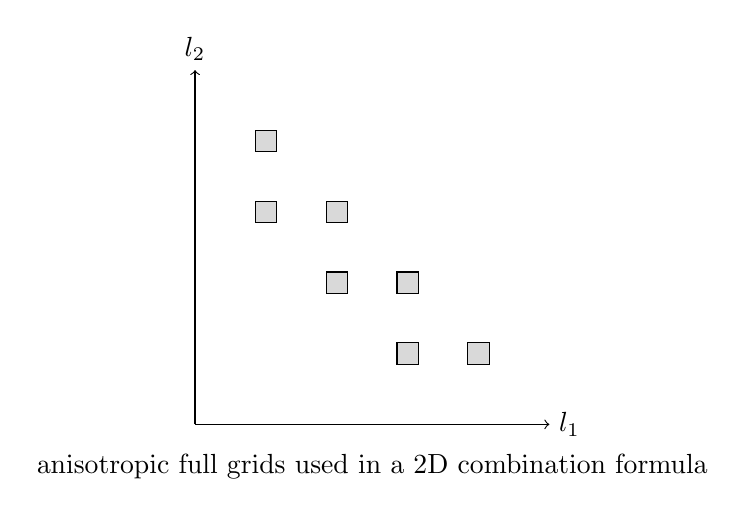
\begin{tikzpicture}[scale=0.9]
\draw[->] (0,0) -- (5,0) node[right] {$l_1$};
\draw[->] (0,0) -- (0,5) node[above] {$l_2$};

\foreach \x/\y in {1/3,2/2,3/1,1/4,2/3,3/2,4/1}
  \draw[fill=gray!30] (\x-0.15,\y-0.15) rectangle (\x+0.15,\y+0.15);

\node at (2.5,-0.6) {anisotropic full grids used in a 2D combination formula};
\end{tikzpicture}
\caption{Schematic of the combination-technique viewpoint: the sparse-grid approximation is reconstructed from several anisotropic full-grid solves.}
\label{fig:combination}
\end{figure}

\section{Algorithmic realization}

A generic direct sparse-grid interpolation/discretization pipeline is:

\begin{algorithm}[ht]
\caption{Classical sparse-grid construction and use}
\begin{algorithmic}[1]
\Require Dimension $d$, maximal level $n$, one-dimensional hierarchical basis
\State Construct all multi-indices $l\in\mathbb{N}^d$ with $|l|_1\le n+d-1$
\ForAll{active levels $l$}
  \State Build the anisotropic subspace $W_l$
  \State Enumerate its odd-grid basis functions $\{\phi_{l,i}\}_{i\in I_l}$
\EndFor
\State Form the sparse basis $\{\phi_\lambda\}_{\lambda\in\Lambda_n}$ of $\widehat V_n$
\If{interpolation}
  \State Compute hierarchical surpluses $v_{l,i}$ from nodal values
  \State Return $\widehat u_n=\sum_{\lambda\in\Lambda_n} v_\lambda \phi_\lambda$
\Else
  \State Assemble sparse-grid matrices $M,K,\ldots$ in the basis $\{\phi_\lambda\}$
  \State Solve the resulting linear system or time-stepping sequence
\EndIf
\end{algorithmic}
\label{alg:sg}
\end{algorithm}

For PDEs, the main additional tasks are:
\begin{itemize}
\item assembling bilinear forms on sums of anisotropic tensor spaces,
\item designing fast matrix-vector products and preconditioners,
\item handling adaptivity when the mixed-regularity assumption is only locally valid.
\end{itemize}

\section{Adaptivity, higher order, and limitations}

Sparse grids are not restricted to piecewise linear approximation. One may use:
\begin{itemize}
\item higher-order hierarchical Lagrange bases,
\item interpolets,
\item prewavelets and wavelets.
\end{itemize}
Higher-order bases improve approximation if the solution is smoother, while wavelet-type bases offer better stability properties and more robust coefficient-based error estimation.

Sparse grids also admit local adaptivity. In practice, one often refines based on weighted hierarchical surpluses, thereby restoring efficiency for localized singularities or anisotropic layers.

Still, sparse grids are not universally appropriate. They rely on the idea that the solution has enough mixed regularity. If the solution contains severe corner singularities, shocks, strongly localized ridges not aligned with coordinate axes, or highly irregular coefficients, then the asymptotic sparse-grid advantage may deteriorate substantially unless adaptive or problem-tailored modifications are used.

\section{Take-away for parabolic PDEs}

For diffusion-like parabolic PDEs, sparse grids provide a spatial discretization whose cost is dramatically smaller than that of a full tensor-product method, while retaining good approximation properties under mixed regularity. In the energy norm especially, the method is theoretically and practically well aligned with the variational structure of diffusion operators. This is why sparse grids appear naturally in high-dimensional heat equations, Fokker--Planck equations, and some Schr\"odinger-type settings after suitable reformulation.

%%%%%%%%%%%%%%%%%%%%%%%%%%%%%%%%%%%%%%%%%%%%%%%%%%%%%%%%%%%%%%%%%%%%%%%%%%%%%%
\chapter{Applying sparse grids to a concrete PDE: a 5D heat equation}

\section{Model problem}

We now work out in detail how one applies a sparse-grid discretization to a concrete five-dimensional parabolic PDE. Let
$$
\Omega := (0,1)^5,
\qquad
T>0.
$$
Consider
\begin{equation}
\partial_t u(x,t) - \nabla\cdot\bigl(a(x)\nabla u(x,t)\bigr) = f(x,t),
\qquad (x,t)\in \Omega\times(0,T],
\label{eq:heat}
\end{equation}
with homogeneous Dirichlet boundary conditions
$$
u(x,t)=0,
\qquad x\in\partial\Omega,
$$
and initial condition
$$
u(x,0)=u_0(x), \qquad x\in\Omega.
$$
Assume
$$
0<a_{\min}\le a(x)\le a_{\max}<\infty,
$$
with $a$ sufficiently smooth, say $a\in W^{1,\infty}(\Omega)$, and assume $f$ and $u_0$ are smooth enough that the solution has the mixed regularity needed by the sparse-grid approximation theory.

A concrete example is
$$
a(x)=1+\frac12\sum_{j=1}^5 x_j,
\qquad
f(x,t)=e^{-t}\prod_{j=1}^5 \sin(\pi x_j).
$$
Nothing in the sparse-grid construction depends on this specific choice; it just fixes the coefficients.

\section{Weak formulation}

Let
$$
V:=H_0^1(\Omega).
$$
Multiply \eqref{eq:heat} by a test function $v\in V$, integrate over $\Omega$, and integrate the diffusion term by parts. Since $v=0$ on $\partial\Omega$, the boundary term vanishes and we obtain:
find $u:[0,T]\to V$ such that
\begin{equation}
(\partial_t u(t),v) + a_\Omega(u(t),v) = (f(t),v)
\qquad \forall v\in V,\quad t\in(0,T],
\label{eq:weak}
\end{equation}
where
$$
a_\Omega(w,v)
:=
\int_\Omega a(x)\,\nabla w(x)\cdot \nabla v(x)\,dx.
$$
Because $a(x)\ge a_{\min}>0$, the bilinear form is coercive:
$$
a_\Omega(v,v)\ge a_{\min}\|\nabla v\|_{L^2(\Omega)}^2.
$$
Hence the natural norm is the weighted energy norm
$$
\|v\|_{E,a}
:=
\bigl(a_\Omega(v,v)\bigr)^{1/2},
$$
which is equivalent to the usual $H_0^1$-seminorm.

\section{Sparse-grid space in $d=5$}

Choose a sparse-grid level $n$. For each multi-index $l=(l_1,\dots,l_5)\in\mathbb{N}^5$, define the anisotropic increment space $W_l$ exactly as in the general theory. Then the classical five-dimensional sparse-grid space is
$$
\widehat V_n
=
\bigoplus_{|l|_1\le n+4} W_l.
$$
The number of degrees of freedom satisfies
$$
\dim \widehat V_n
=
\sum_{i=0}^{n-1} 2^i \binom{4+i}{4}
=
O(2^n n^4),
$$
whereas the corresponding full-grid space of level $n$ would have $O(2^{5n})$ unknowns. This is the central computational gain.

Let
$$
\Lambda_n := \{(l,i): |l|_1\le n+4,\ i\in I_l\}
$$
be the global sparse-grid index set, and let
$$
\{\phi_\lambda\}_{\lambda\in\Lambda_n}
$$
be the associated hierarchical basis functions.

\section{Semidiscrete Galerkin approximation}

We now discretize only in space. Seek
$$
u_n(t)\in \widehat V_n
$$
of the form
$$
u_n(x,t)=\sum_{\lambda\in\Lambda_n} U_\lambda(t)\,\phi_\lambda(x).
$$
Insert this into the weak formulation and test with every basis function $\phi_\mu$, $\mu\in\Lambda_n$. This yields
$$
\sum_{\lambda\in\Lambda_n} \dot U_\lambda(t)\,(\phi_\lambda,\phi_\mu)
+
\sum_{\lambda\in\Lambda_n} U_\lambda(t)\,a_\Omega(\phi_\lambda,\phi_\mu)
=
(f(t),\phi_\mu).
$$
In matrix form:
\begin{equation}
M \dot U(t) + K U(t) = F(t),
\label{eq:semi}
\end{equation}
where
$$
M_{\mu\lambda} := (\phi_\lambda,\phi_\mu)
= \int_\Omega \phi_\lambda(x)\phi_\mu(x)\,dx,
$$
$$
K_{\mu\lambda} := a_\Omega(\phi_\lambda,\phi_\mu)
= \int_\Omega a(x)\,\nabla \phi_\lambda(x)\cdot \nabla \phi_\mu(x)\,dx,
$$
$$
F_\mu(t) := (f(t),\phi_\mu).
$$

\subsection{Structure of the matrices}

Because each basis function is a tensor product,
$$
\phi_{l,i}(x)=\prod_{j=1}^5 \phi_{l_j,i_j}(x_j),
$$
one can factor many integrals into sums/products of one-dimensional contributions when $a(x)$ is separable or approximated in separable form. Even for general $a(x)$, the tensor-product structure is valuable algorithmically.

For constant diffusion $a(x)\equiv 1$, the stiffness entry becomes
$$
K_{\mu\lambda}
=
\sum_{m=1}^5
\left(
\prod_{\substack{j=1\\j\ne m}}^5
\int_0^1 \phi_{\lambda,j}(x_j)\phi_{\mu,j}(x_j)\,dx_j
\right)
\left(
\int_0^1 \phi'_{\lambda,m}(x_m)\phi'_{\mu,m}(x_m)\,dx_m
\right).
$$
Thus one can assemble the 5D operator from 1D mass and stiffness building blocks.

\section{Time discretization}

Choose a time step $\tau=T/N_t$ and times $t_m=m\tau$. For diffusion problems, backward Euler is the simplest robust choice. Approximate
$$
\dot U(t_{m+1}) \approx \frac{U^{m+1}-U^m}{\tau}.
$$
Then \eqref{eq:semi} gives
\begin{equation}
(M+\tau K)U^{m+1} = M U^m + \tau F^{m+1},
\label{eq:BE}
\end{equation}
where
$$
F^{m+1}_\mu := \int_\Omega f(x,t_{m+1})\phi_\mu(x)\,dx.
$$
The initial vector $U^0$ is obtained from an $L^2$-projection or interpolation of $u_0$ into $\widehat V_n$.

Backward Euler is first-order in time and unconditionally stable. If higher temporal accuracy is needed, one may use Crank--Nicolson:
$$
\left(M+\frac{\tau}{2}K\right)U^{m+1}
=
\left(M-\frac{\tau}{2}K\right)U^m
+
\frac{\tau}{2}\bigl(F^{m+1}+F^m\bigr).
$$

\section{How the system is constructed in practice}

A practical implementation proceeds as follows.

\subsection{Step 1: generate the active subspaces}

Enumerate all $l\in\mathbb{N}^5$ such that
$$
|l|_1\le n+4.
$$
For each such $l$, enumerate the odd-index grid points
$$
i\in I_l.
$$
This defines the global basis index set $\Lambda_n$.

\subsection{Step 2: build basis-function metadata}

For each basis function $\phi_{l,i}$, store:
\begin{itemize}
\item its level $l$,
\item its grid index $i$,
\item its support box
$$
\operatorname{supp}\phi_{l,i}
=
\prod_{j=1}^5
\bigl[x_{l_j,i_j}-2^{-l_j},\,x_{l_j,i_j}+2^{-l_j}\bigr].
$$
\end{itemize}
Since hat functions are compactly supported, matrix entries vanish unless supports overlap. This is crucial for sparse assembly.

\subsection{Step 3: assemble $M$ and $K$}

For each pair $(\lambda,\mu)$ with overlapping support:
\begin{enumerate}
\item compute $M_{\mu\lambda}$,
\item compute $K_{\mu\lambda}$,
\item add contributions to the global sparse matrix.
\end{enumerate}
In a direct sparse-grid code, one exploits:
\begin{itemize}
\item compact support,
\item tensor-product separability of basis functions,
\item hierarchical indexing,
\item often some variant of the unidirectional principle for efficient operator application.
\end{itemize}

\subsection{Step 4: initial condition}

Either interpolate:
$$
u_n^0 = I_{\widehat V_n}u_0,
$$
or project:
$$
(MU^0)_\mu = (u_0,\phi_\mu).
$$
Projection is usually preferable in a Galerkin setting.

\subsection{Step 5: right-hand side at each step}

For each $m$, compute
$$
F_\mu^{m+1} = \int_\Omega f(x,t_{m+1})\phi_\mu(x)\,dx.
$$
If $f$ is separable in the coordinates, these integrals are cheap. If not, one uses quadrature adapted to the support geometry.

\subsection{Step 6: solve the linear system}

At each time step solve
$$
A_\tau U^{m+1}=b^{m+1},
\qquad
A_\tau:=M+\tau K.
$$
The matrix $A_\tau$ is symmetric positive definite, so one can use:
\begin{itemize}
\item conjugate gradients,
\item multilevel preconditioners,
\item hierarchical diagonal scaling,
\item sparse-grid-specific subspace correction methods.
\end{itemize}

\section{What error to expect}

Assume the exact solution is sufficiently smooth in the mixed sense uniformly in time. Then the sparse-grid spatial approximation behaves, roughly, as follows:
\begin{itemize}
\item in $L^2$: second order in $h_n$, up to a factor $n^{4}$ in $d=5$,
\item in energy norm: first order in $h_n$,
\item with degrees of freedom $O(2^n n^4)$ instead of $O(2^{5n})$.
\end{itemize}
Thus the sparse grid replaces a catastrophic $5$-fold tensor growth by a nearly one-dimensional growth times a polynomial-in-$n$ correction.

For the fully discrete scheme with backward Euler, the total error typically splits into
$$
\text{space error} + \text{time error}
\approx
O(h_n |\log h_n|^{4}) \ \text{in energy norm}
\quad+\quad O(\tau).
$$
So one should balance $\tau$ with the spatial accuracy.

\section{Direct sparse-grid discretization versus combination technique}

For this 5D heat equation, there are two main implementation routes.

\subsection{Route A: direct sparse-grid FEM}

Use the space $\widehat V_n$ exactly as above and solve \eqref{eq:BE}. This is mathematically clean and matches the variational formulation directly.

\subsection{Route B: combination technique}

Instead of constructing $\widehat V_n$ explicitly, solve the semidiscrete or fully discrete heat equation on anisotropic full grids corresponding to levels $l$ with
$$
n\le |l|_1 \le n+4,
$$
and combine these full-grid solutions with the appropriate alternating binomial coefficients. This often reuses standard solvers on tensor-product grids and is especially attractive on parallel architectures.

\section{What changes for Fokker--Planck or Schr\"odinger-type equations?}

The sparse-grid machinery in space is largely unchanged. What changes is:
\begin{itemize}
\item the bilinear form,
\item possible non-symmetry (for drift terms),
\item conservation or positivity constraints,
\item the preferred time integrator.
\end{itemize}
For Fokker--Planck equations, one adds drift terms and may need stabilization or conservative formulations. For Schr\"odinger-type equations, the operator becomes indefinite or complex-valued, and one often prefers different bases and time stepping. But the sparse-grid idea --- hierarchical tensor-product truncation under mixed regularity --- remains the same.

\section{Final practical interpretation}

For a 5D heat equation, sparse grids are best viewed as a structured reduction of tensor-product resolution. One still resolves each coordinate direction hierarchically, but one refuses to pay for the simultaneously finest scales in all directions. If the solution truly has bounded mixed derivatives and no violent cross-dimensional singular structure, this gives a deterministic high-dimensional discretization that is vastly cheaper than a full grid while preserving the natural energy-norm accuracy relevant to diffusion problems.

\end{document}